%
% Frontmatter - Introducci�n. Los miembros del tribunal que juzgan los PFC's tienen muchas m�s memorias que leer, por lo que
%	agradecer�n cualquier detalle que permita facilitarles la vida. En este sentido, realizar una peque�a introducci�n,
%	comentar la organizaci�n y estructura de la memoria y resumir brevemente cada cap�tulo puede ser una buena pr�ctica
%	que permita al lector centrarse f�cilmente en la parte que m�s le interesa.
%

\chapter[Introduction]{
	Introduction
}

Computer Vision is a field that includes techniques for acquiring, processing, analyzing, and understanding images. This scientific area is not only limited to images but also to high-dimensional data from the real world. It aims to produce numerical or symbolic information in order to perform decisions \cite{computervision}. A common trend in this field, has been duplicating the abilities of human vision by electronically perceiving and interpreting the image. 

\begin{figure}[h]
	\centering
	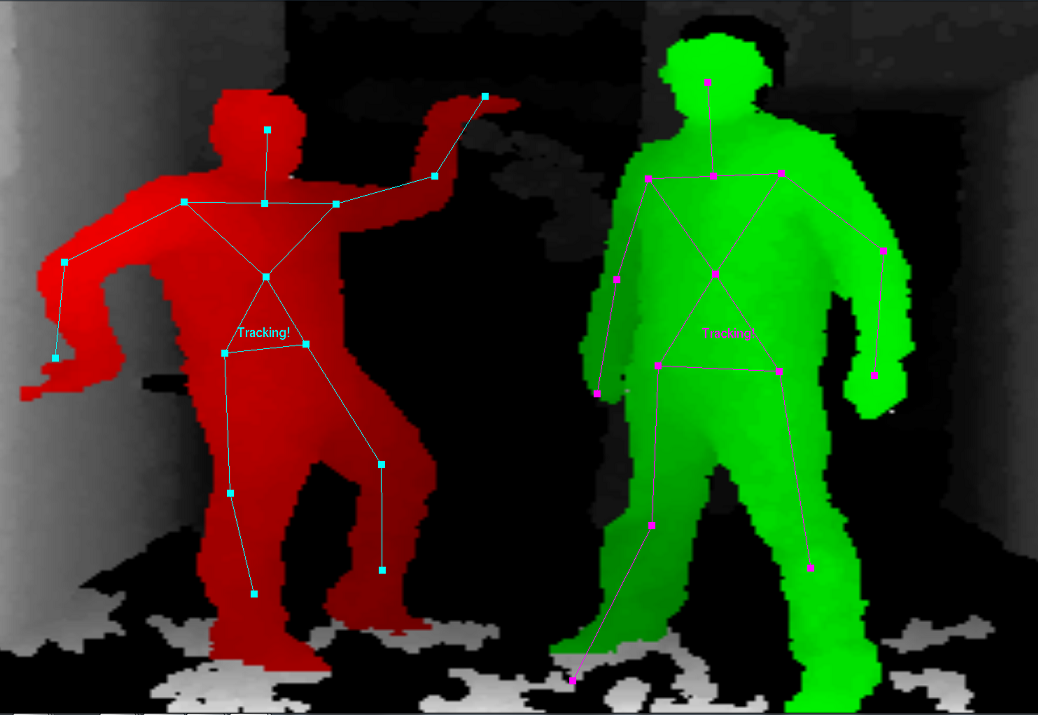
\includegraphics[scale=0.4]{figures/pose_estimation.png}
	\caption[Pose estimation]{
		The specific task of determining the pose of an object in an image is referred to as pose estimation.
	}
	\label{pose_estimation}
\end{figure}

This image understanding can be seen as the extraction of symbolic information from image data using models constructed with the aid of geometry, physics, statistics, and learning theory \cite{computervisionmodern}. As a scientific discipline, Computer Vision considers the theory behind artificial systems that extract information from images. The image data can have many forms, such as video frames, views from multiple cameras, or multi-dimensional data from a medical scanner. As a technological discipline, Computer Vision seeks to apply its theories and models to the construction of artificial vision systems.

Sub-domains of computer vision include scene reconstruction, event detection, video tracking, object recognition, object pose estimation, learning, indexing, motion estimation, and image restoration (see \figurename~\ref{pose_estimation}). Our case study pertains to the field of stereo vision. In this subject, the main objective is the extraction of 3D information from digital images, such as obtained by a CCD camera. By comparing information about a scene from two vantage points, 3D data can be extracted by examination of the relative positions of objects in the two panels (see \figurename~\ref{stereoscopic_vision}).

\begin{figure}[h]
  \centering
  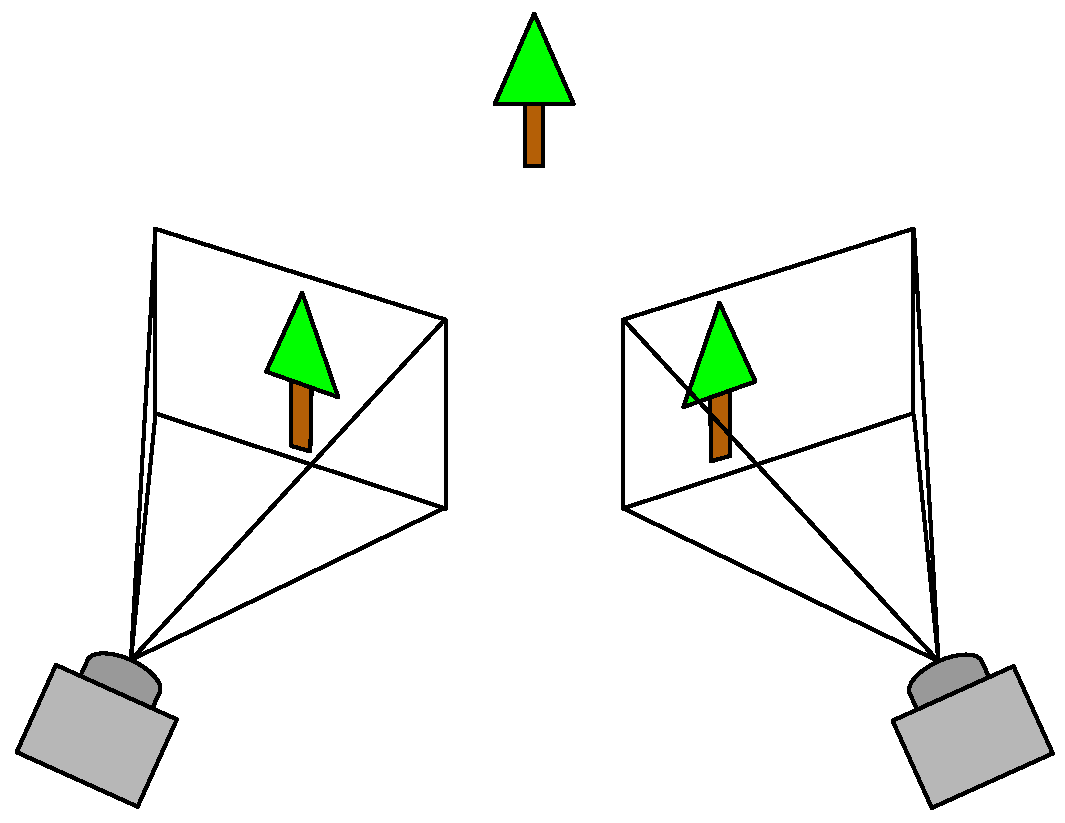
\includegraphics[width=0.475\textwidth]{figures/stereo.pdf} \quad
  \caption[Stereoscopic vision]{
  		Basic diagram of a stereo vision setup.
  	}
  \label{stereoscopic_vision}
\end{figure} 

\section[Motivation and context]{
	Project motivation and context
}

One of the key steps in stereo vision techniques, is obtaining the stereo correspondence between two images or Stereo Matching. The correspondence problem refers to the process of ascertaining which parts of one image correspond to which parts of another image. This is not a trivial affair, since differences appear due to movement of the camera, the elapse of time, and/or movement of objects in the photos.

Current approaches to obtain this information, involve the usage of a single CPU. Our aim with this project is taking advantage of modern hardware to its fullest capacities. This is specially important nowadays, since camera systems keep on improving leading to images with very high resolutions. This complex task involves exploiting the massive parallel power of current multi-core CPUs, GPUs, etc. In addition, our desire is not only the implementation of a Stereo Matching algorithm; but the creation of a \CC framework that will allow the user to implement parallel Computer Vision algorithms with ease.

The set of software tools developed in this project has been called \textbf{GCVL} (GPU Computer Vision Library). This library provides several means to implement GPU algorithms in an simpler manner. 

\section[Objectives]{
	Project objectives
}

The aim of this project is the design and implementation of a point-based multi-platform software tool for the interactive visualization, management, analysis and manipulation of massive 3D point clouds. 

The application will offer the user the necessary tools to work effectively with this type of datasets, including a 3D visualizer with advanced point-rendering techniques using OpenGL, that will allow real time interaction with one or multiple point clouds.

From the interface, the user will be able to:

\begin{itemize}
\item Select different visualization modes for point-based models: multiple cameras, simple and advanced visualization, multi-resolution, etc.
\item Combine different point clouds with tools that enable rotation, translation and scaling of the datasets.
\item Select points in the clouds for working with them.
\item Apply operations to a part of the cloud or the complete dataset. From simple operations, such as distance measurement and calculation, to plane or other geometric primitives detection.
\item Export the work done to a standard CAD format, so the tool can be integrated in other work-flows.
\item Call the pre- and post-processing tools included in the suite: multi-resolution structure computation, filters, etc.
\end{itemize}

The developed tool will take advantage of the parallel computing possibilities of the platforms. Both using the GPGPU capabilities of the graphics card with OpenCL and the multiple cores of the CPU. 

PCM will be used as the foundation for this work. PCM is a project in development that offers several low level tools for working with point clouds of arbitrary size in commodity hardware, from which a multi-resolution structure with different levels of cache is highlighted. This final degree project will not only extend PCM with the mentioned features, offering a high level software suite for the final user, but will also improve the existing source code, paying special attention to performance aspects.

A series of benchmarks will also be implemented that will allow us to obtain automatically and autonomously performance information about PCM and the visualization tool, with graphs and reports. This tool will make finding bottlenecks and performance issues easier.

\section[Structure]{
Document structure
}

The rest of the document is organized following this structure:

\paragraph*{Chapter 2.}
Planning and methodology

After this introduction, we start by describing the planning and
development methodology used in the project. We chose an agile
software development approach.

\paragraph*{Chapter 3.}
Computer Graphics basics

This chapter briefs the very basic concepts about computer graphics needed to understand the rest of the document: How a virtual camera works and the different types of cameras, what 3D transformations are and how a point is represented in 3D.
 
\paragraph*{Chapter 4.}
Structure of a real-time visualizer for point-based datasets

This chapter describes the structure of the visualizer we propose in this work and presents the class diagram of the software package. Both ToView (the visualization tool) and PCM (the multi-resolution library behind the GUI) are included.

\paragraph*{Chapter 5.}
Point Cloud Manager

This chapter focussed in describing PCM ant detailing all the work
invested in the improvement of the original PCM library and tools:
code refactoring, bug fixes and new functionalities. It includes the
experimental results of the tests included in the benchmarks we have
designed to measure the library performance.

\paragraph*{Chapter 6.}
ToView

This chapter depicts the visualizer designed and implemented from
scratch in this project to manage and visualize massive point
clouds. All the included functionalities are described and
experimental results are also included.

\paragraph*{Chapter 7.}
Advanced GPU point rendering

This chapter is devoted to the most advanced visualization methods
included in ToView, a bunch of some of the most state-of-the-art
point-rendering techniques, and how they are implemented with OpenGL
in the GPU using GLSL (OpenGL Shading Language).

\paragraph*{Chapter 8.}
Object detection: RANSAC

This chapter deals with the detection of different shapes and volumes
in ToView, describing the different approaches that were studied to implement
this functionality in the project. Specifically, an extensive
explanation of the RANSAC algorithms used in this project is provided.

\paragraph*{Chapter 9.}
Preprocessing and filtering

Both PCM and ToView need several pre-processing tasks to take advantage
of some of the most advances features. All this pre-processing and the
different filtering techniques applied to the datasets are explored in
this chapter.

\paragraph*{Chapter 10.}
Conclusions and future lines of work

Finally, this chapter presents the main conclusions obtained with this
project and outlines possible extensions to both PCM and ToView.
